\chapter{経路と閉路 - Paths and circuits}

この章では次の2つの経路を扱います。
\begin{itemize}
\item \key{オイラー路 - Eulerian path} 各辺をちょうど1回ずつ通る経路
\item \key{ハミルトン路 - Hamiltonian path} 各ノードをちょうど1回ずつ訪れる経路
\end{itemize}

一見、オイラー経路とハミルトン経路は似た経路に見えますが全く異なったものです。
グラフにオイラー経路があるかどうかは非常に簡単なルールがあり、
オイラー経路がある場合にそれを見つける効率的なアルゴリズムが存在します。
しかし、ハミルトンパスの存在を確認することは、 NP困難(NP-Hard)な問題で、
この問題を解くための効率的なアルゴリズムは知られていません。

\section{オイラー路 - Eulerian paths}

\index{オイラー路 - Eulerian path}

\key{オイラー路 - Eulerian path}\footnote{L. Euler studied such paths in 1736
when he solved the famous Königsberg bridge problem.
This was the birth of graph theory.} はグラフの各辺をちょうど1回ずつ通る経路です。
\begin{center}
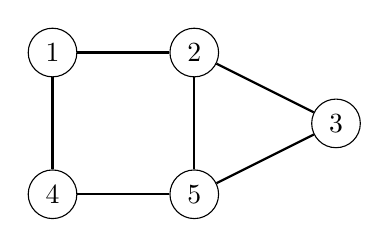
\begin{tikzpicture}[scale=0.9]
\node[draw, circle] (1) at (1,5) {$1$};
\node[draw, circle] (2) at (3,5) {$2$};
\node[draw, circle] (3) at (5,4) {$3$};
\node[draw, circle] (4) at (1,3) {$4$};
\node[draw, circle] (5) at (3,3) {$5$};

\path[draw,thick,-] (1) -- (2);
\path[draw,thick,-] (2) -- (3);
\path[draw,thick,-] (1) -- (4);
\path[draw,thick,-] (3) -- (5);
\path[draw,thick,-] (2) -- (5);
\path[draw,thick,-] (4) -- (5);
\end{tikzpicture}
\end{center}
このグラフはノード2からノード5までのオイラー路を持ちます。
\begin{center}
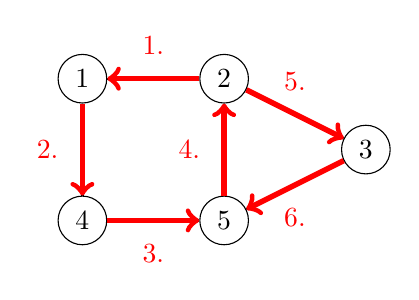
\begin{tikzpicture}[scale=0.9]
\node[draw, circle] (1) at (1,5) {$1$};
\node[draw, circle] (2) at (3,5) {$2$};
\node[draw, circle] (3) at (5,4) {$3$};
\node[draw, circle] (4) at (1,3) {$4$};
\node[draw, circle] (5) at (3,3) {$5$};

\path[draw,thick,-] (1) -- (2);
\path[draw,thick,-] (2) -- (3);
\path[draw,thick,-] (1) -- (4);
\path[draw,thick,-] (3) -- (5);
\path[draw,thick,-] (2) -- (5);
\path[draw,thick,-] (4) -- (5);

\path[draw=red,thick,->,line width=2pt] (2) -- node[font=\small,label={[red]north:1.}] {} (1);
\path[draw=red,thick,->,line width=2pt] (1) -- node[font=\small,label={[red]left:2.}] {} (4);
\path[draw=red,thick,->,line width=2pt] (4) -- node[font=\small,label={[red]south:3.}] {} (5);
\path[draw=red,thick,->,line width=2pt] (5) -- node[font=\small,label={[red]left:4.}] {} (2);
\path[draw=red,thick,->,line width=2pt] (2) -- node[font=\small,label={[red]north:5.}] {} (3);
\path[draw=red,thick,->,line width=2pt] (3) -- node[font=\small,label={[red]south:6.}] {} (5);
\end{tikzpicture}
\end{center}
\index{オイラー閉路 - Eulerian circuit}
\key{オイラー閉路 - Eulerian circuit}
とは、同じノードで始まり、同じノードで終わるオイラー路です。
\begin{center}
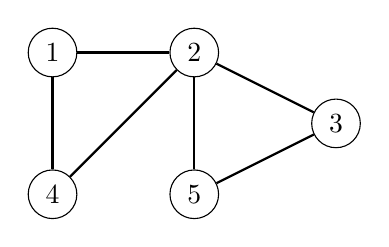
\begin{tikzpicture}[scale=0.9]
\node[draw, circle] (1) at (1,5) {$1$};
\node[draw, circle] (2) at (3,5) {$2$};
\node[draw, circle] (3) at (5,4) {$3$};
\node[draw, circle] (4) at (1,3) {$4$};
\node[draw, circle] (5) at (3,3) {$5$};

\path[draw,thick,-] (1) -- (2);
\path[draw,thick,-] (2) -- (3);
\path[draw,thick,-] (1) -- (4);
\path[draw,thick,-] (3) -- (5);
\path[draw,thick,-] (2) -- (5);
\path[draw,thick,-] (2) -- (4);
\end{tikzpicture}
\end{center}
このグラフでは以下のようなノード1開始のオイラー閉路を持ちます。
\begin{center}
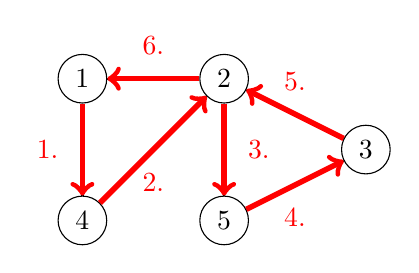
\begin{tikzpicture}[scale=0.9]
\node[draw, circle] (1) at (1,5) {$1$};
\node[draw, circle] (2) at (3,5) {$2$};
\node[draw, circle] (3) at (5,4) {$3$};
\node[draw, circle] (4) at (1,3) {$4$};
\node[draw, circle] (5) at (3,3) {$5$};

\path[draw,thick,-] (1) -- (2);
\path[draw,thick,-] (2) -- (3);
\path[draw,thick,-] (1) -- (4);
\path[draw,thick,-] (3) -- (5);
\path[draw,thick,-] (2) -- (5);
\path[draw,thick,-] (2) -- (4);

\path[draw=red,thick,->,line width=2pt] (1) -- node[font=\small,label={[red]left:1.}] {} (4);
\path[draw=red,thick,->,line width=2pt] (4) -- node[font=\small,label={[red]south:2.}] {} (2);
\path[draw=red,thick,->,line width=2pt] (2) -- node[font=\small,label={[red]right:3.}] {} (5);
\path[draw=red,thick,->,line width=2pt] (5) -- node[font=\small,label={[red]south:4.}] {} (3);
\path[draw=red,thick,->,line width=2pt] (3) -- node[font=\small,label={[red]north:5.}] {} (2);
\path[draw=red,thick,->,line width=2pt] (2) -- node[font=\small,label={[red]north:6.}] {} (1);
\end{tikzpicture}
\end{center}

\subsubsection{存在の判定 - Existence}

オイラー路と閉路の存在はノードの次数によって判定できます。
無向グラフにおいてオイラー路を持つのはすべての辺が同じ連結成分に属し、

\begin{itemize}
\item 全てのノードの次数が偶数
\item ちょうど2つのノードだけの次数が奇数で他のすべてのノードの次数が偶数
\end{itemize}

この2つのどちらか一方を満たしている場合である。

最初の場合に各オイラー路はオイラー閉路でもあります。

2番目の場合は奇数次ノードの2つのオイラーパスの始点と終点になります。
次のグラフを例にします。

\begin{samepage}
\begin{center}
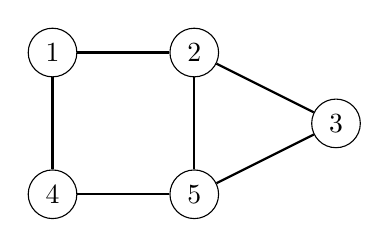
\begin{tikzpicture}[scale=0.9]
\node[draw, circle] (1) at (1,5) {$1$};
\node[draw, circle] (2) at (3,5) {$2$};
\node[draw, circle] (3) at (5,4) {$3$};
\node[draw, circle] (4) at (1,3) {$4$};
\node[draw, circle] (5) at (3,3) {$5$};

\path[draw,thick,-] (1) -- (2);
\path[draw,thick,-] (2) -- (3);
\path[draw,thick,-] (1) -- (4);
\path[draw,thick,-] (3) -- (5);
\path[draw,thick,-] (2) -- (5);
\path[draw,thick,-] (4) -- (5);
\end{tikzpicture}
\end{center}
\end{samepage}

ノード1、3、4は次数2でノード2、5が次数3で、ちょうど2つのノードが奇数の次数を持ちます。
ノード2と5の間にはオイラー経路が存在するが、
このグラフにはオイラー閉路は存在しません。

有向グラフでは、ノードの出次数と入次数に注目します。
有向グラフにおいてオイラー路を正確に含むのは、
すべての辺が同じ連結成分に所属しておりかつ、

\begin{itemize}
\item 全てのノードにおいて出次数と入次数が等しい
\item ある一つのノードで入次数が出次数より1だけ大きく、他の一つのノードで出次数が入次数より1だけ大きく、
他の全てのノードでは出次数と入次数が等しい
\end{itemize}

この2つの条件のどちらかを満たしているグラフである必要があります。
最初の条件を満たす場合、存在するオイラー路はオイラー閉路でもあります。
2つ目の条件を満たす場合、開始を出次数が大きなノードとして、
終了を入次が大きなノードとしたオイラー閉路が存在します。

以下のようなグラフを考えます。
\begin{center}
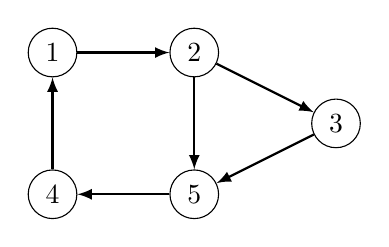
\begin{tikzpicture}[scale=0.9]
\node[draw, circle] (1) at (1,5) {$1$};
\node[draw, circle] (2) at (3,5) {$2$};
\node[draw, circle] (3) at (5,4) {$3$};
\node[draw, circle] (4) at (1,3) {$4$};
\node[draw, circle] (5) at (3,3) {$5$};

\path[draw,thick,->,>=latex] (1) -- (2);
\path[draw,thick,->,>=latex] (2) -- (3);
\path[draw,thick,->,>=latex] (4) -- (1);
\path[draw,thick,->,>=latex] (3) -- (5);
\path[draw,thick,->,>=latex] (2) -- (5);
\path[draw,thick,->,>=latex] (5) -- (4);
\end{tikzpicture}
\end{center}

ノード1、3、4はともに入次数と出次数は1です。
ノード2は入次数1で出次数は2で、
ノード5は入次数2で出次数は1です。
このため、次のようにノード2からノード5へのオイラー路が存在することがわかります。

\begin{center}
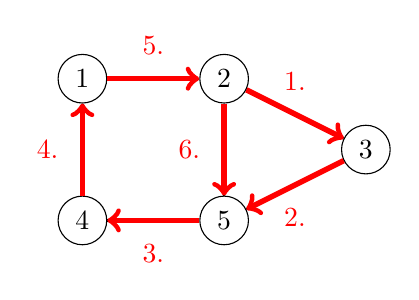
\begin{tikzpicture}[scale=0.9]
\node[draw, circle] (1) at (1,5) {$1$};
\node[draw, circle] (2) at (3,5) {$2$};
\node[draw, circle] (3) at (5,4) {$3$};
\node[draw, circle] (4) at (1,3) {$4$};
\node[draw, circle] (5) at (3,3) {$5$};

\path[draw,thick,-] (1) -- (2);
\path[draw,thick,-] (2) -- (3);
\path[draw,thick,-] (1) -- (4);
\path[draw,thick,-] (3) -- (5);
\path[draw,thick,-] (2) -- (5);
\path[draw,thick,-] (4) -- (5);

\path[draw=red,thick,->,line width=2pt] (2) -- node[font=\small,label={[red]north:1.}] {} (3);
\path[draw=red,thick,->,line width=2pt] (3) -- node[font=\small,label={[red]south:2.}] {} (5);
\path[draw=red,thick,->,line width=2pt] (5) -- node[font=\small,label={[red]south:3.}] {} (4);
\path[draw=red,thick,->,line width=2pt] (4) -- node[font=\small,label={[red]left:4.}] {} (1);
\path[draw=red,thick,->,line width=2pt] (1) -- node[font=\small,label={[red]north:5.}] {} (2);
\path[draw=red,thick,->,line width=2pt] (2) -- node[font=\small,label={[red]left:6.}] {} (5);
\end{tikzpicture}
\end{center}

\subsubsection{ヒールホルツァーのアルゴリズム - Hierholzer's algorithm}

\index{ヒールホルツァーのアルゴリズム - Hierholzer's algorithm}

\key{ヒールホルツァーのアルゴリズム - Hierholzer's algorithm}\footnote{The algorithm was published
in 1873 after Hierholzer's death \cite{hie73}.}
は、オイラー閉路を構築する効率的なアルゴリズムです。
このアルゴリズムはグラフに閉路が存在することを前提として、
複数のラウンドを実行し、各ラウンドは閉路となる新しい辺を追加していきます。

まず、グラフの辺の一部(全てでなくてもよい)を含む回路を構築します。
その後、この閉路に別の閉路を追加することにより、段階的に回路を拡張していきます。
これをすべての辺が閉路に追加されるまで繰り返します。

このアルゴリズムは閉路に属しているノードで
閉路に含まれていない出次辺を持つノード$x$を処理して閉路を拡張していきます。
このノード$x$から、まだ閉路に含まれていないエッジのみを含む新しい経路を構築します。
いずれそのパスはノード$x$に戻り、サブ閉路が作られる。

もし、グラフにオイラー路しかない場合でも、
グラフに余分な辺を追加し、閉路を構築した後にその辺を削除すれば、
ヒールホルツァーのアルゴリズムで路を求めることができます。
例えば、無向グラフの場合は2つの奇数次ノードの間に余分なエッジを追加します

実際にヒールホルツァーのアルゴリズムが無向グラフに対し、
どのようにオイラー路を構築するかを見ていきましょう。

\subsubsection{Example}

\begin{samepage}
\begin{center}
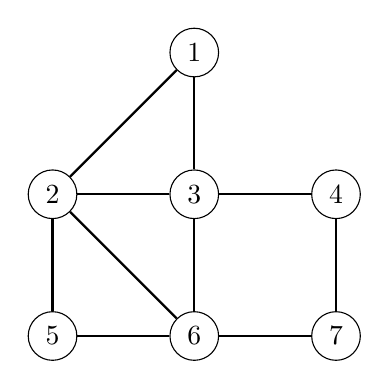
\begin{tikzpicture}[scale=0.9]
\node[draw, circle] (1) at (3,5) {$1$};
\node[draw, circle] (2) at (1,3) {$2$};
\node[draw, circle] (3) at (3,3) {$3$};
\node[draw, circle] (4) at (5,3) {$4$};
\node[draw, circle] (5) at (1,1) {$5$};
\node[draw, circle] (6) at (3,1) {$6$};
\node[draw, circle] (7) at (5,1) {$7$};

\path[draw,thick,-] (1) -- (2);
\path[draw,thick,-] (1) -- (3);
\path[draw,thick,-] (2) -- (3);
\path[draw,thick,-] (2) -- (5);
\path[draw,thick,-] (2) -- (6);
\path[draw,thick,-] (3) -- (4);
\path[draw,thick,-] (3) -- (6);
\path[draw,thick,-] (4) -- (7);
\path[draw,thick,-] (5) -- (6);
\path[draw,thick,-] (6) -- (7);
\end{tikzpicture}
\end{center}
\end{samepage}

\begin{samepage}
まずノード1から始まる回路を作成するとします。
たとえば$1 \rightarrow 2 \rightarrow 3 \rightarrow 1$です。

\begin{center}
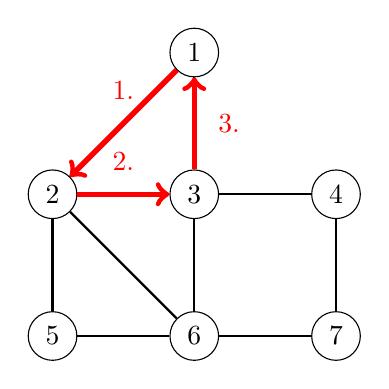
\begin{tikzpicture}[scale=0.9]
\node[draw, circle] (1) at (3,5) {$1$};
\node[draw, circle] (2) at (1,3) {$2$};
\node[draw, circle] (3) at (3,3) {$3$};
\node[draw, circle] (4) at (5,3) {$4$};
\node[draw, circle] (5) at (1,1) {$5$};
\node[draw, circle] (6) at (3,1) {$6$};
\node[draw, circle] (7) at (5,1) {$7$};

\path[draw,thick,-] (1) -- (2);
\path[draw,thick,-] (1) -- (3);
\path[draw,thick,-] (2) -- (3);
\path[draw,thick,-] (2) -- (5);
\path[draw,thick,-] (2) -- (6);
\path[draw,thick,-] (3) -- (4);
\path[draw,thick,-] (3) -- (6);
\path[draw,thick,-] (4) -- (7);
\path[draw,thick,-] (5) -- (6);
\path[draw,thick,-] (6) -- (7);

\path[draw=red,thick,->,line width=2pt] (1) -- node[font=\small,label={[red]north:1.}] {} (2);
\path[draw=red,thick,->,line width=2pt] (2) -- node[font=\small,label={[red]north:2.}] {} (3);
\path[draw=red,thick,->,line width=2pt] (3) -- node[font=\small,label={[red]east:3.}] {} (1);
\end{tikzpicture}
\end{center}
\end{samepage}
このあと、部分閉路である
$2 \rightarrow 5 \rightarrow 6 \rightarrow 2$を追加していきます。

\begin{center}
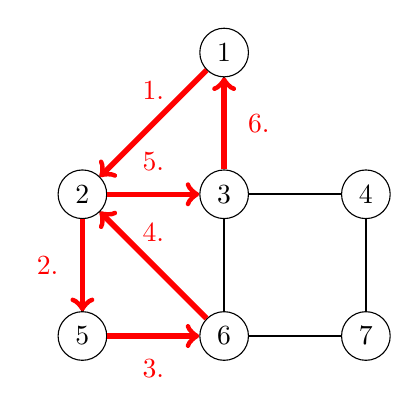
\begin{tikzpicture}[scale=0.9]
\node[draw, circle] (1) at (3,5) {$1$};
\node[draw, circle] (2) at (1,3) {$2$};
\node[draw, circle] (3) at (3,3) {$3$};
\node[draw, circle] (4) at (5,3) {$4$};
\node[draw, circle] (5) at (1,1) {$5$};
\node[draw, circle] (6) at (3,1) {$6$};
\node[draw, circle] (7) at (5,1) {$7$};

\path[draw,thick,-] (1) -- (2);
\path[draw,thick,-] (1) -- (3);
\path[draw,thick,-] (2) -- (3);
\path[draw,thick,-] (2) -- (5);
\path[draw,thick,-] (2) -- (6);
\path[draw,thick,-] (3) -- (4);
\path[draw,thick,-] (3) -- (6);
\path[draw,thick,-] (4) -- (7);
\path[draw,thick,-] (5) -- (6);
\path[draw,thick,-] (6) -- (7);

\path[draw=red,thick,->,line width=2pt] (1) -- node[font=\small,label={[red]north:1.}] {} (2);
\path[draw=red,thick,->,line width=2pt] (2) -- node[font=\small,label={[red]west:2.}] {} (5);
\path[draw=red,thick,->,line width=2pt] (5) -- node[font=\small,label={[red]south:3.}] {} (6);
\path[draw=red,thick,->,line width=2pt] (6) -- node[font=\small,label={[red]north:4.}] {} (2);
\path[draw=red,thick,->,line width=2pt] (2) -- node[font=\small,label={[red]north:5.}] {} (3);
\path[draw=red,thick,->,line width=2pt] (3) -- node[font=\small,label={[red]east:6.}] {} (1);
\end{tikzpicture}
\end{center}
そして、
$6 \rightarrow 3 \rightarrow 4 \rightarrow 7 \rightarrow 6$
を追加します。
\begin{center}
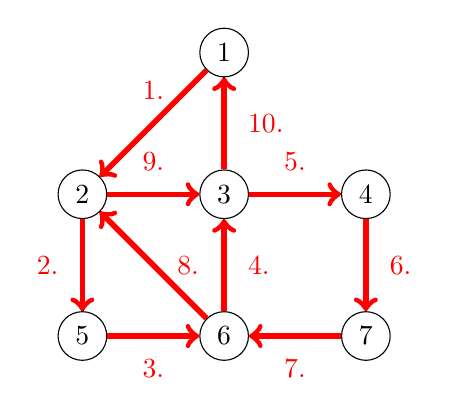
\begin{tikzpicture}[scale=0.9]
\node[draw, circle] (1) at (3,5) {$1$};
\node[draw, circle] (2) at (1,3) {$2$};
\node[draw, circle] (3) at (3,3) {$3$};
\node[draw, circle] (4) at (5,3) {$4$};
\node[draw, circle] (5) at (1,1) {$5$};
\node[draw, circle] (6) at (3,1) {$6$};
\node[draw, circle] (7) at (5,1) {$7$};

\path[draw,thick,-] (1) -- (2);
\path[draw,thick,-] (1) -- (3);
\path[draw,thick,-] (2) -- (3);
\path[draw,thick,-] (2) -- (5);
\path[draw,thick,-] (2) -- (6);
\path[draw,thick,-] (3) -- (4);
\path[draw,thick,-] (3) -- (6);
\path[draw,thick,-] (4) -- (7);
\path[draw,thick,-] (5) -- (6);
\path[draw,thick,-] (6) -- (7);

\path[draw=red,thick,->,line width=2pt] (1) -- node[font=\small,label={[red]north:1.}] {} (2);
\path[draw=red,thick,->,line width=2pt] (2) -- node[font=\small,label={[red]west:2.}] {} (5);
\path[draw=red,thick,->,line width=2pt] (5) -- node[font=\small,label={[red]south:3.}] {} (6);
\path[draw=red,thick,->,line width=2pt] (6) -- node[font=\small,label={[red]east:4.}] {} (3);
\path[draw=red,thick,->,line width=2pt] (3) -- node[font=\small,label={[red]north:5.}] {} (4);
\path[draw=red,thick,->,line width=2pt] (4) -- node[font=\small,label={[red]east:6.}] {} (7);
\path[draw=red,thick,->,line width=2pt] (7) -- node[font=\small,label={[red]south:7.}] {} (6);
\path[draw=red,thick,->,line width=2pt] (6) -- node[font=\small,label={[red]right:8.}] {} (2);
\path[draw=red,thick,->,line width=2pt] (2) -- node[font=\small,label={[red]north:9.}] {} (3);
\path[draw=red,thick,->,line width=2pt] (3) -- node[font=\small,label={[red]east:10.}] {} (1);
\end{tikzpicture}
\end{center}
これによってオイラー閉路が完成しました。

\section{ハミルトン路 - Hamiltonian paths}

\index{ハミルトン路 - Hamiltonian path}

\key{ハミルトン路 - Hamiltonian path}
というのは各ノードをちょうど1回ずつ訪問するパスのことです。

\begin{center}
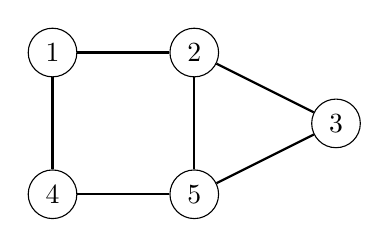
\begin{tikzpicture}[scale=0.9]
\node[draw, circle] (1) at (1,5) {$1$};
\node[draw, circle] (2) at (3,5) {$2$};
\node[draw, circle] (3) at (5,4) {$3$};
\node[draw, circle] (4) at (1,3) {$4$};
\node[draw, circle] (5) at (3,3) {$5$};

\path[draw,thick,-] (1) -- (2);
\path[draw,thick,-] (2) -- (3);
\path[draw,thick,-] (1) -- (4);
\path[draw,thick,-] (3) -- (5);
\path[draw,thick,-] (2) -- (5);
\path[draw,thick,-] (4) -- (5);
\end{tikzpicture}
\end{center}
これはノード1からノード3というハミルトン路があります。
\begin{center}
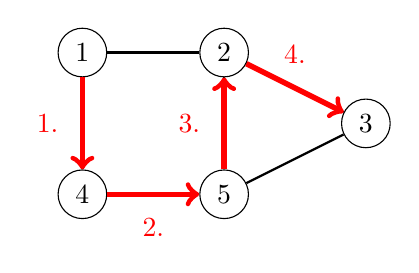
\begin{tikzpicture}[scale=0.9]
\node[draw, circle] (1) at (1,5) {$1$};
\node[draw, circle] (2) at (3,5) {$2$};
\node[draw, circle] (3) at (5,4) {$3$};
\node[draw, circle] (4) at (1,3) {$4$};
\node[draw, circle] (5) at (3,3) {$5$};

\path[draw,thick,-] (1) -- (2);
\path[draw,thick,-] (2) -- (3);
\path[draw,thick,-] (1) -- (4);
\path[draw,thick,-] (3) -- (5);
\path[draw,thick,-] (2) -- (5);
\path[draw,thick,-] (4) -- (5);

\path[draw=red,thick,->,line width=2pt] (1) -- node[font=\small,label={[red]left:1.}] {} (4);
\path[draw=red,thick,->,line width=2pt] (4) -- node[font=\small,label={[red]south:2.}] {} (5);
\path[draw=red,thick,->,line width=2pt] (5) -- node[font=\small,label={[red]left:3.}] {} (2);
\path[draw=red,thick,->,line width=2pt] (2) -- node[font=\small,label={[red]north:4.}] {} (3);
\end{tikzpicture}
\end{center}

\index{ハミルトン閉路 - Hamiltonian circuit}

ハミルトン路が同じノードで始まり、同じノードで終わるような経路を
ハミルトン閉路と呼びます。
上のグラフにはノード1から始まりノード1で終わるハミルトン閉路があります。

\begin{center}
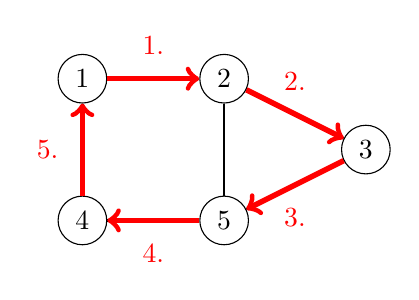
\begin{tikzpicture}[scale=0.9]
\node[draw, circle] (1) at (1,5) {$1$};
\node[draw, circle] (2) at (3,5) {$2$};
\node[draw, circle] (3) at (5,4) {$3$};
\node[draw, circle] (4) at (1,3) {$4$};
\node[draw, circle] (5) at (3,3) {$5$};

\path[draw,thick,-] (1) -- (2);
\path[draw,thick,-] (2) -- (3);
\path[draw,thick,-] (1) -- (4);
\path[draw,thick,-] (3) -- (5);
\path[draw,thick,-] (2) -- (5);
\path[draw,thick,-] (4) -- (5);

\path[draw=red,thick,->,line width=2pt] (1) -- node[font=\small,label={[red]north:1.}] {} (2);
\path[draw=red,thick,->,line width=2pt] (2) -- node[font=\small,label={[red]north:2.}] {} (3);
\path[draw=red,thick,->,line width=2pt] (3) -- node[font=\small,label={[red]south:3.}] {} (5);
\path[draw=red,thick,->,line width=2pt] (5) -- node[font=\small,label={[red]south:4.}] {} (4);
\path[draw=red,thick,->,line width=2pt] (4) -- node[font=\small,label={[red]left:5.}] {} (1);
\end{tikzpicture}
\end{center}

\subsubsection{存在の確認}

グラフにハミルトン路が含まれるかどうかを調べる効率的な方法は知られておらず、この問題はNP-Hardです。
しかし、いくつかのケースでグラフがハミルトン路を含んでいることがわかっています。

単純な考察からわかるのはグラフが完全である場合、
すなわちすべてのノードのペアの間にエッジがある場合には
ハミルトン路も含んでいることになります。
さらにいくつかの証明もされています。

\begin{itemize}
\item
\index{ディラックの定理 - Dirac's theorem}
\key{ディラックの定理 - Dirac's theorem}: %\cite{dir52}
全てのノードが$n/2$以上の次数である場合、グラフにはハミルトン路が存在する
\item
\index{オレの定理 - Ore's theorem}
\key{オレの定理 - Ore's theorem}: %\cite{ore60}
隣接しない全てのペアの次数の和が$n$以上である場合、グラフにはハミルトン路が存在する
\end{itemize}

これらに共通する性質は、
グラフが多数の辺を持つ場合にハミルトンパスの存在を保証しています。
これは、グラフに含まれる辺の数が多いほど、
ハミルトン路を構成する可能性が高いので理にかなっています。

\subsubsection{構築 - Construction}

そもそもハミルトン路が存在するかどうかを判定する効率的な方法がないため、
パスを効率的に構築する方法もありません。
パスが構築できるなら、それが存在するかどうかを確認すればよいです。

さて、ハミルトンパスを探索する最もシンプルな方法は、
パスを構成する可能なすべての方法を調べるバックトラックのアルゴリズムを使用することです。
ただし、このアルゴリズムの時間計算量は少なくとも$O(n!)$です。

より効率的な解決策は動的計画法に基づいていて実現できます(10.5章参照)。
このアイデアは、関数$\texttt{possible}(S,x)$の値を計算することす。
ここで$S$はノードの部分集合、$x$はノードの1つとします。
この関数は、$S$のノードを訪れ、
ノード$x$で 終わるハミルトンパスが存在するかどうかを判定します。
この解法は$O(2^n n^2)$時間で実装できます。

\section{デ・ブルーイェン配列 - De Bruijn sequences}

\index{デ・ブルーイェン配列 - De Bruijn sequence}

\key{デ・ブルーイェン配列 - De Bruijn sequence}
は、文字数$k$の固定アルファベットの文字列に対して、
長さ$n$のすべての文字列を部分文字列として
ちょうど一度だけ含む文字列のことです。
このような文字列の長さは$k^n+n-1$文字です。
例えば、$n = 3$, $k = 2$ のときにDe Bruijn配列の例は次のようになります。
\[0001011100.\]
これは以下のような全ての部分文字列を含みます。
000, 001, 010, 011, 100, 101, 110, 111.

De Bruijn配列は、グラフのオイラー路に対応することが分かっています。
そこで、各ノードが$n - 1$文字の文字列を含み、
各辺がその文字列に1 文字ずつ追加するグラフを作成します。
次のグラフは、上記のシナリオに対応するグラフです。

\begin{center}
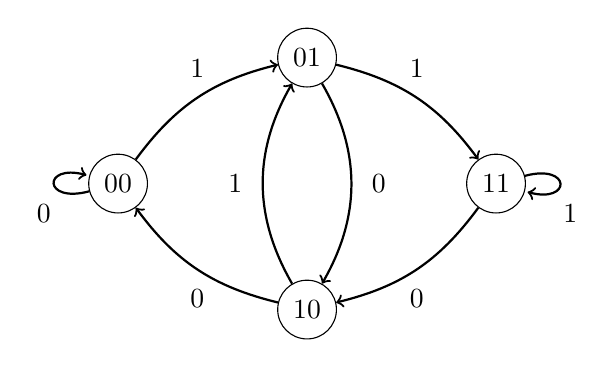
\begin{tikzpicture}[scale=0.8]
\node[draw, circle] (00) at (-3,0) {00};
\node[draw, circle] (11) at (3,0) {11};
\node[draw, circle] (01) at (0,2) {01};
\node[draw, circle] (10) at (0,-2) {10};

\path[draw,thick,->] (00) edge [bend left=20] node[font=\small,label=1] {} (01);
\path[draw,thick,->] (01) edge [bend left=20] node[font=\small,label=1] {} (11);
\path[draw,thick,->] (11) edge [bend left=20] node[font=\small,label=below:0] {} (10);
\path[draw,thick,->] (10) edge [bend left=20] node[font=\small,label=below:0] {} (00);

\path[draw,thick,->] (01) edge [bend left=30] node[font=\small,label=right:0] {} (10);
\path[draw,thick,->] (10) edge [bend left=30] node[font=\small,label=left:1] {} (01);

\path[draw,thick,-] (00) edge [loop left] node[font=\small,label=below:0] {} (00);
\path[draw,thick,-] (11) edge [loop right] node[font=\small,label=below:1] {} (11);
\end{tikzpicture}
\end{center}

このグラフのオイラー路は、
長さnの文字列をすべて含む文字列に対応します。
この文字列には開始ノードの文字とエッジの文字がすべて含まれています。
始点ノードは$n - 1$文字でエッジには$k^n$文字があるため、
文字列の長さは$k^n+n-1$となります。

\section{ナイトツアー - Knight's tours}

\index{ナイトツアー - knight's tour}

\key{ナイトツアー - knight's tour}は$n \times n$のチェス盤上で、
チェスのルールに従って騎士(ナイト)が各マスにちょうど1回ずつ訪れるような動き
のことです。
ナイトツアーは,
最終的にスタート地点のマスに戻る場合はクローズドツアー,
そうでない場合 はオープンツアーと呼ばれます。
例えば、$5 \times 5$ボードのオープンナイトのツアーを示します。

\begin{center}
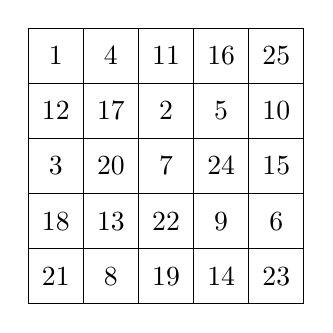
\begin{tikzpicture}[scale=0.7]
\draw (0,0) grid (5,5);
\node at (0.5,4.5) {$1$};
\node at (1.5,4.5) {$4$};
\node at (2.5,4.5) {$11$};
\node at (3.5,4.5) {$16$};
\node at (4.5,4.5) {$25$};
\node at (0.5,3.5) {$12$};
\node at (1.5,3.5) {$17$};
\node at (2.5,3.5) {$2$};
\node at (3.5,3.5) {$5$};
\node at (4.5,3.5) {$10$};
\node at (0.5,2.5) {$3$};
\node at (1.5,2.5) {$20$};
\node at (2.5,2.5) {$7$};
\node at (3.5,2.5) {$24$};
\node at (4.5,2.5) {$15$};
\node at (0.5,1.5) {$18$};
\node at (1.5,1.5) {$13$};
\node at (2.5,1.5) {$22$};
\node at (3.5,1.5) {$9$};
\node at (4.5,1.5) {$6$};
\node at (0.5,0.5) {$21$};
\node at (1.5,0.5) {$8$};
\node at (2.5,0.5) {$19$};
\node at (3.5,0.5) {$14$};
\node at (4.5,0.5) {$23$};
\end{tikzpicture}
\end{center}

ナイトツアーは、
盤上のマスをノードとしたグラフのハミルトン路といえます。
ナイトがチェスのルールに従ってマスの間を移動できる場合、
2つのノードを辺で結びます。

ナイトツアーを構成する一般的な方法はバックトラックを使うことです。
完全なツアーを素早く見つけるためにはヒューリスティックを用いると効率的です。

\subsubsection{ウォーンスドルフの法則 - Warnsdorf's rule}

\index{ヒューリスティック - heuristic}
\index{ウォーンスドルフの法則 - Warnsdorf's rule}

\key{ウォーンスドルフの法則}\footnote{This heuristic was proposed
in Warnsdorf's book \cite{war23} in 1823. There are
also polynomial algorithms for finding knight's tours
\cite{par97}, but they are more complicated.}
は、ナイトのツアーを見つけるためのシンプルで効果的手法です。
この法則を用いると、$n$が大きな盤面でも効率的にツアーを構成することができます。
この法則は移動可能なマスの数ができるだけ少なくなるように、
常にナイトを移動させていきます。

次のような状況で、
ナイトが移動できるマスは5つあります(squares $a \ldots e$)。
\begin{center}
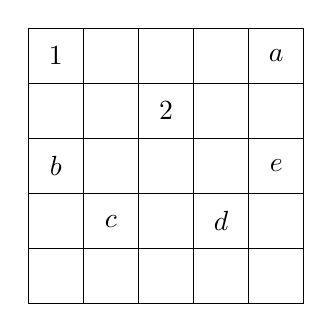
\begin{tikzpicture}[scale=0.7]
\draw (0,0) grid (5,5);
\node at (0.5,4.5) {$1$};
\node at (2.5,3.5) {$2$};
\node at (4.5,4.5) {$a$};
\node at (0.5,2.5) {$b$};
\node at (4.5,2.5) {$e$};
\node at (1.5,1.5) {$c$};
\node at (3.5,1.5) {$d$};
\end{tikzpicture}
\end{center}

この場合、ウォーンスドルフのルールでは、ナイトをaマスに移動させます。
この選択の後は1手しかないためです。
他の選択肢では3手まで可能なマスにナイトを移動させることができます。